% ----------------------------------------
% ----------------------------------------
% Presentation template
% Author: Miloš D. Petrašinović <mpetrasinovic@mas.bg.ac.rs>
% Faculty of Mechanical Engineering, University of Belgrade
% Department of Aerospace Engineering, Flying structures
% https://vazmfb.com
% Belgrade, 2021
% ----------------------------------------
% ----------------------------------------

% ----------------------------------------
% Used packages definition and document format
% ----------------------------------------
\documentclass[12pt]{beamer}
\usetheme{_vazmfb}
\usepackage[T1]{fontenc}
\usepackage[utf8]{inputenc}
\usepackage{tikz}
\usepackage{ulem}
\usepackage{lineno}
\usepackage{hyperref}
\usepackage{subcaption}
\usepackage{textcomp}
\usepackage{setspace}
\usepackage{gensymb}
\usepackage[numbered]{matlab-prettifier}
\usepackage{graphicx}
\usepackage[english]{babel}
\usepackage{placeins}
\usepackage{amssymb}
\usepackage{amsmath}
\usepackage[toc,title]{appendix}
\usepackage{nomencl}
\usepackage{float}
\usepackage{caption}
\usepackage{bigstrut}
\usepackage{booktabs}
\usepackage{colortbl}
\usepackage{multirow}
\usepackage{multicol}
\usepackage{siunitx}
\usepackage{array}
\usepackage{fancyvrb}
\usepackage{icomma}
\usepackage{lmodern}
\usepackage{listings}
\usepackage{diagbox}
\usepackage{bm}
\usepackage[numbered]{matlab-prettifier}

% Folder for figures
\graphicspath{{figures/}}

% Colors
\definecolor{tamno-plava}{cmyk}{1,0.79,0.32,0.17}
\definecolor{svetlo-plava}{cmyk}{0.93,0.64,0.03,0}
\definecolor{siva}{cmyk}{0.73,0.67,0.65,0.8}
\definecolor{tamno-siva}{HTML}{aaaaaa}
\definecolor{zelena}{cmyk}{1,0,1,0.5}

% Enumerations
\newcommand\itemS{\item[\textbf{\S}]}

% Matrix 
\makeatletter
\renewcommand*\env@matrix[1][c]{\hskip -\arraycolsep
  \let\@ifnextchar\new@ifnextchar
  \array{*\c@MaxMatrixCols #1}}
\makeatother

% Matlab code
\lstset{
  style = Matlab-editor,
  basicstyle = \fontfamily{pcr}\selectfont\footnotesize, % if you want to use Courier
  numberstyle = \tiny\color{siva},
  commentstyle = \color{zelena},
}

% Units of measurement
\sisetup{
  per-mode=fraction,
  fraction-function=\tfrac
}

% Norms
\newcommand{\norm}[1]{\left\lVert#1\right\rVert}
\newcommand{\abs}[1]{\left\lvert#1\right\rvert}
\newcommand{\diff}[1]{\mathrm{d}#1}

% Font
\usefonttheme{default}
%\usefonttheme{serif}

% No continuation in the next row
\tolerance=1
\emergencystretch=\maxdimen
\hyphenpenalty=10000
\hbadness=10000

%----------------------------------
% INPUT DATA
%----------------------------------

\title[Course title]{Course title} % Enter course title
\subtitle{Presentation title} % Enter presentation title
\date{10.12.2021.} % Enter presentation date
\institute[Department of Aerospace Engineering]{\textbf{Department of Aerospace Engineering} \\ Faculty of Mechanical Engineering \\ University of Belgrade}
\authorsgroup{\orcid{First name Last Name}{0000-0000-0000-0000}} % Replace first and last name and 0000-0000-0000-0000 with ORCID
\webpage{vazmfb.com/course/} % Replace the course with the course address

\webpageurl{https://vazmfb.com/course/} % Replace the course with the course address

% ----------------------------------------
% BEGINNING OF THE DOCUMENT
% ----------------------------------------
\begin{document}

% ----------------------------------------
% FIRST FRAME
% ----------------------------------------
{
	\setbeamertemplate{headline}{}
	\setbeamertemplate{footline}{}
	\maketitle
}
\addtocounter{framenumber}{-1} % without counting the first page

% ----------------------------------------
% Section
% ----------------------------------------
\section{Section title}

% ----------------------------------------
% FRAME
% ----------------------------------------
\begin{frame}{Slide title}

Inserting an image (image \ref{orao}) into the presentation % Referencing with \label and \ref

\begin{figure}
    \centering
    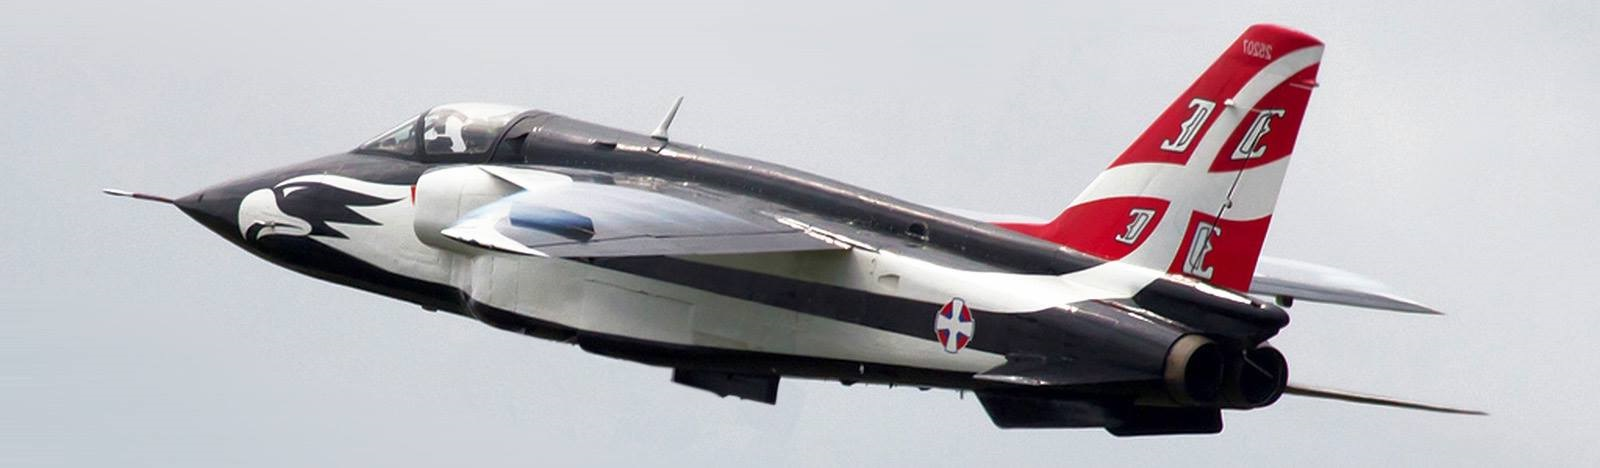
\includegraphics[width=0.9\textwidth]{orao}
    \caption{Figure captiom}
    \label{orao}
\end{figure}
\end{frame}

% ----------------------------------------
% FRAME
% ----------------------------------------
\begin{frame}{}
Lists and two columns on slide

\vspace{1cm} % vertical distance

% Left half
\begin{minipage}{0.49\textwidth}
    \begin{itemize}
    	\item First 
    	\item Second
    	\item Third
    \end{itemize}
\end{minipage}
% Right half
\begin{minipage}{0.49\textwidth}
    \begin{enumerate}
    	\item First 
    	\item Second
    	\item Third
    \end{enumerate}
\end{minipage}

\vspace{1cm} % vertical distance

\textit{Website address with link:} % Italic text
\url{https://vazmfb.com}

\href{https://vazmfb.com}{Text with link to vazmfb.com}

\end{frame}

% ----------------------------------------
% FRAME
% ----------------------------------------
\begin{frame}{New slide title}
\begin{vazmfb_block}{Definition title}
    Definition text
\end{vazmfb_block}

Equation \ref{eq1} % The equation and all other elements are referenced in the same way
\begin{equation}
    \label{eq1}
    \Pi = \frac{1}{2} \int_{V} \bm{\varepsilon}^T\, \bm{\sigma}\, \text{d}V = \frac{1}{2} \int_{V} \bm{\varepsilon}^T\, \bm{c}\, \bm{\varepsilon}\, \diff{V}
\end{equation}

\end{frame}

% ----------------------------------------
% FRAME
% ----------------------------------------
\begin{frame}{}


Program example:
\lstinputlisting[language=Matlab, caption=Program caption]{programs/program.m}

Example of \textbf{matrix equations} % Bold text
\footnotesize
\begin{equation}
    \begin{bmatrix}
       \sigma_{xx} \\
       \sigma_{yy} \\
       \sigma_{zz} \\
       \sigma_{yz} \\
       \sigma_{xz} \\
       \sigma_{xy} \\
    \end{bmatrix} 
     = 
    \begin{bmatrix}
       c_{11} & c_{12} & c_{13} & c_{14} & c_{15} & c_{16} \\
       & c_{22} & c_{23} & c_{24} & c_{25} & c_{26} \\
       & & c_{33} & c_{34} & c_{35} & c_{36} \\
       & & & c_{44} & c_{45} & c_{46} \\
       & & & & c_{55} & c_{56} \\
       \multicolumn{2}{c}{\text{Sim.}} & & & & c_{66} \\
    \end{bmatrix} 
    \begin{bmatrix}
       \varepsilon_{xx} \\
       \varepsilon_{yy} \\
       \varepsilon_{zz} \\
       \gamma_{yz} \\
       \gamma_{xz} \\
       \gamma_{xy} \\
    \end{bmatrix} 
\end{equation}

\end{frame}

% ----------------------------------------
% FRAME
% ----------------------------------------
\begin{frame}{}

Example table

\begin{table}[H]
\large
\centering
\caption{Table caption}
\begin{tabular}[H]{|l|c|}
\hline
First cell & Right \\ \hline
Down & Diagonal \\ \hline
\end{tabular}
\end{table}
\end{frame}

\section{End of presentation}
% ----------------------------------------
% FRAME
% ----------------------------------------
\begin{frame}
\centering
\Huge Thank you for your attention!
\end{frame}

% ----------------------------------------
% END OF DOCUMENT
% ----------------------------------------
\end{document}